\begin{figure}
\begin{tabular}{@{}c@{}c@{}c@{}}
\begin{subfigure}[b]{0.32\textwidth}
\begin{center}
{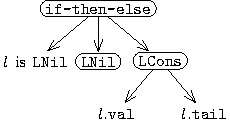
\includegraphics[scale=1.3]{chapters/figures/figUnifTreeListVar.pdf}}
\end{center}
\vspace{4px}
\caption{\label{fig:uniftreelistvar}\sumIf{\sumIs{l}{LNil}} \sumThen{\cons{LNil}} \\ \qquad\quad \sumElse{\cons{LCons}(\prodAccess{l}{val},\prodAccess{l}{tail})}}
\end{subfigure}%
&
\begin{subfigure}[b]{0.32\textwidth}
\begin{center}
{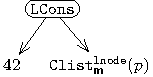
\includegraphics[scale=1.3]{chapters/figures/figUnifTreeCons.pdf}}
\end{center}
\vspace{28px}
\caption{\label{fig:uniftreecons}\cons{LCons}(42, \lifted{list}{\mem{}}{lnode}{p})}
\end{subfigure}%
&
\begin{subfigure}[b]{0.32\textwidth}
\begin{center}
{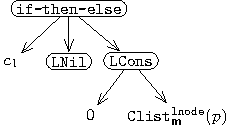
\includegraphics[scale=1.3]{chapters/figures/figUnifTreeIte.pdf}}
\end{center}
\caption{\label{fig:uniftreeite}\sumIf{c_1} \sumThen{\cons{LNil}} \\ \qquad \sumElse{\cons{LCons}(0, l)}}
\end{subfigure}%
\\
\end{tabular}
\caption{\label{fig:uniftrees}Expression trees corresponding to three \type{List} expressions used in the context of unification of expressions in \cref{sec:unifyandrewrite}.}
\end{figure}
